\newpage
\section{Class \tkzClass{line}} %(fold)

The variable \tkzVar{line}{L} holds a table used to store line objects. It is optional, and users are free to choose their own variable name (e.g., \tkzname{Lines}).
However, for consistency and readability, it is recommended to use \tkzVar{line}{L}. The function \tkzFct{tkz-elements}{init\_elements()} reinitializes this table automatically.


\subsection{Creating a Line}
\label{sub:creating_a_line}

To define a line passing through two known points, use the following constructor:

\begin{mybox}
  \code{L.AB = line(z.A, z.B)} \hfill (short form, recommended)\\
  \code{L.AB = line:new(z.A, z.B)} \hfill (explicit form)
\end{mybox}

This creates a line object \code{L.AB} representing:
\begin{itemize}
  \item the infinite line passing through points \code{z.A} and \code{z.B}, and
  \item the segment $[AB]$, which is used to compute attributes such as the midpoint or direction.
\end{itemize}

\medskip
\noindent
Internally, this object stores the two defining points and derives several geometric properties from them.

\subsection{Attributes of a line} %(fold)

Let's consider  |L.AB = line(z.A, z.B)|

A line object provides access to the following attributes:

\vspace{1em}
\bgroup
  \small
  \captionof{table}{Line attributes.}\label{line:attributes}
  \begin{tabular}{lll}
  \toprule
  \textbf{Attribute}   & \textbf{Meaning} & \textbf{Reference}\\
  \midrule
  \tkzAttr{line}{type} & Always \code{"line"}           &           \\
  \tkzAttr{line}{pa}   & First point (e.g., \code{z.A})   &           \\
  \tkzAttr{line}{pb}   & Second point (e.g., \code{z.B})  &           \\
  \tkzAttr{line}{mid}  & Midpoint of segment $[AB]$     &           \\
  \tkzAttr{line}{slope}& Angle with respect to the horizontal axis & [\ref{ssub:example_class_line}] \\
  \tkzAttr{line}{length} & Euclidean distance $AB$ &  \ref{ssub:example_class_line}] \\
  \tkzAttr{line}{vec}   & Vector $B - A$  &  [\ref{sec:class_vector}] \\
  \tkzAttr{line}{north\_pa}  & Auxiliary point north of \code{pa} & [\ref{ssub:example_class_line}]  \\
    \tkzAttr{line}{north\_pb} & Auxiliary point north of \code{pb} & -- \\
    \tkzAttr{line}{south\_pa} & Auxiliary point south of \code{pa} & -- \\
    \tkzAttr{line}{south\_pb} & Auxiliary point south of \code{pb} & -- \\
    \tkzAttr{line}{east}      & Auxiliary point east of the segment & -- \\
    \tkzAttr{line}{west}      & Auxiliary point west of the segment & -- \\
  \bottomrule
  \end{tabular}
\egroup


\subsubsection{Example: attributes of class line} %(fold)
\label{ssub:example_class_line}

\vspace{1em}
\begin{minipage}{.5\textwidth}
\directlua{
  init_elements()
  z.a = point(1, 1)
  z.b = point(5, 4)
  L.ab = line(z.a, z.b)
  z.m = L.ab.mid
  z.w = L.ab.west
  z.e = L.ab.east
  z.r = L.ab.north_pa
  z.s = L.ab.south_pb
  sl = L.ab.slope
  len = L.ab.length}
\begin{center}
\begin{tikzpicture}[scale = .5 ]
   \tkzGetNodes
   \tkzDrawPoints(a,b,m,e,r,s,w)
   \tkzLabelPoints(a,b)
   \tkzLabelPoint(r){north\_pa}
   \tkzLabelPoint(s){south\_pb}
   \tkzLabelPoint[below](m){mid}
   \tkzLabelPoint[right](w){west}
   \tkzLabelPoint[left](e){east}
   \tkzDrawLine(a,b)
   \tkzLabelSegment[above = 1em,sloped](a,b){ab = \pmpn{\tkzUseLua{len}}}
   \tkzLabelSegment[above=2em,sloped](a,b){slope of(ab) =  \pmpn{\tkzUseLua{sl}}}
\end{tikzpicture}
\end{center}
\end{minipage}
\begin{minipage}{.5\textwidth}
\begin{tkzexample}[code only]
\directlua{
  init_elements()
  z.a = point(1, 1)
  z.b = point(5, 4)
  L.ab = line(z.a, z.b)
  z.m = L.ab.mid
  z.w = L.ab.west
  z.e = L.ab.east
  z.r = L.ab.north_pa
  z.s = L.ab.south_pb
  sl = L.ab.slope
  len = L.ab.length}
\end{tkzexample}
\end{minipage}

\subsubsection{Note on line object attributes}

To recover the original defining points of a line object \tkzname{L.name}, use either of the following:

\begin{itemize}
  \item via the method \code{get(n)}, as in \code{z.A, z.B = L.name:get()} See [\ref{ssub:method_line_get},
  \item or directly via its attributes \code{L.name.pa} and \code{L.name.pb}.
\end{itemize}
\newpage

\subsection{Methods of the class line} %(fold)

Here's the list of methods for the \tkzNameObj{line} object. The results can be real numbers, points, lines, circles or triangles. The triangles obtained are similar to the triangles defined below.

\begin{minipage}{\textwidth}
\bgroup
  \catcode`_=12
  \small
  \captionof{table}{Methods of the class line.(part 1)}\label{line:methods part 1}
\begin{tabular}{ll}
\toprule
\textbf{Methods} & \textbf{Reference}  \\
\midrule
    \textbf{Constructor} & \\
    \tkzMeth{line}{new(pt, pt)} &Note\footnote{line(pt, pt) (short form, recommended)}; [\ref{sub:creating_a_line}; \ref{ssub:method_line_new_pt_pt}; \ref{sub:altshiller}] \\

  \midrule
  \textbf{Real-valued Methods} & \\
  \midrule
  \tkzMeth{line}{distance(pt)}  &  [\ref{ssub:method_line_distance}] \\
  \midrule
    \textbf{Boolean Methods} & \\
  \midrule
  \tkzMeth{line}{in\_out(pt)}  & [\ref{ssub:method_in_out};\ref{ssub:in_out_for_a_line}] \\
  \tkzMeth{line}{in\_out\_segment(pt)} & [\ref{ssub:method_line_in_out_segment}] \\
 \tkzMeth{line}{on\_line(pt)}  & idem \\
 \tkzMeth{line}{on\_segment(pt)} & idem \\
 \tkzMeth{line}{is\_parallel(L)}  & [\ref{ssub:method_line_is_parallel}]  \\
  \tkzMeth{line}{is\_orthogonal(L)}  & [\ref{ssub:method_line_is_orthogonal}] \\
  \tkzMeth{line}{is\_equidistant(pt)}  & [\ref{ssub:method_line_is_equidistant}] \\
\midrule

\textbf{Points Methods} & \\
  \midrule
  \tkzMeth{line}{get(n)}     & [\ref{ssub:method_line_get}] \\

 \tkzMeth{line}{random()}     & [  \ref{ssub:method_line_random}] \\

  \tkzMeth{line}{gold\_ratio()}  &  [\ref{ssub:methode_imeth_line_gold__ratio}; \ref{sub:gold_ratio_with_segment} ; \ref{sub:the_figure_pappus_circle} ; \ref{sub:bankoff_circle} ]  \\

\tkzMeth{line}{normalize()}  &  [ \ref{ssub:normalize}]  \\

\tkzMeth{line}{normalize\_inv()}  & [\ref{ssub:normalize}]\\

\tkzMeth{line}{barycenter(r,r)}    &   [\ref{ssub:barycenter_with_a_line}] \\

\tkzMeth{line}{point(r)}   &   [\ref{sub:ellipse} ; \ref{ssub:method_point}] \\

\tkzMeth{line}{midpoint()}    & [\ref{ssub:method_line_midpoint}]  \\

\tkzMeth{line}{harmonic\_int(pt)}   &  [\ref{ssub:method_line_harmonic_int};  \ref{sub:bankoff_circle}] \\

\tkzMeth{line}{harmonic\_ext(pt)}  & [ \ref{sub:bankoff_circle}] \\

\tkzMeth{line}{harmonic\_both(r)}  & [\ref{ssub:harmonic_both}; \ref{ssub:harmonic_division_with_tkzphi}] \\

\tkzMeth{line}{report(d,pt)}    &[\ref{ssub:method_report}]\\

\tkzMeth{line}{colinear\_at(pt,k)}  & [ex. \ref{ssub:method_line_colinear__at}]\\
  \midrule

    \textbf{Line Constructors} & \\
  \midrule

\tkzMeth{line}{ll\_from(pt)}  & [\ref{ssub_line_from_a_defined_line}] \\

\tkzMeth{line}{ortho\_from(pt)} & [\ref{ssubline_ortho_from}] \\

\tkzMeth{line}{mediator()} & Note  Note\footnote{You may use \tkzMeth{perpendicular\_bisector} as a synonym.} ; [\ref{ssub:method_line_mediator}]\\

\tkzMeth{line}{swap\_line()}  & [\ref{ssub:method_line_swap__line} ; \ref{ssub:intersection_line_parabola_explained}] \\

\tkzMeth{line}{orthogonal\_at()} & \ref{ssub:method_line_orthogonal__at} \\
  \midrule


\textbf{Triangle Constructors} & \\
\midrule
\tkzMeth{line}{equilateral(<'swap'>)}    &  Note\footnote{By default, triangles are oriented positively (counter-clockwise). Use \code{"swap"} for clockwise orientation.};  [\ref{ssub:method_line_equilateral};  \ref{ssub:object_rotation}]  \\

\tkzMeth{line}{isosceles(d,<'swap'>)}& [\ref{ssub:method_line_isosceles}]\\

\tkzMeth{line}{two\_angles(an,an)} &Note \footnote{The given side is between the two angles} [\ref{ssub:triangle_with_two__angles}] \\

\tkzMeth{line}{school(<'swap'>)}   &[\ref{ssub:method_imeth_line_school_swap}] \\

\tkzMeth{line}{half(<'swap'>)}      & [\ref{ssub:method_imeth_line_half_swap}]\\

\tkzMeth{line}{s\_s(r,r<,'swap'>)}  &  [\ref{ssub:triangle_with_three_given_sides}] \\

\tkzMeth{line}{sa\_(r,an<,'swap'>)}  &  [\ref{ssub:_line_sas_d_an}]  \\

  \tkzMeth{line}{\_as(r,an<,'swap'>)}  &  [\ref{ssub:_line__as_d_an_swap}]  \\

  \tkzMeth{line}{a\_s(r,an<,'swap'>)}  &  [\ref{ssub:_line_a__s_d_an_swap}]\\

  \tkzMeth{line}{s\_a(r,an<,'swap'>)}  &  [\ref{ssub:_line_sa}]\\
  \bottomrule
  \end{tabular}
  \egroup


\end{minipage}

\begin{minipage}{\textwidth}

\bgroup
\catcode`_=12
\small
\captionof{table}{Methods of the class line.(part 2)}\label{line:methods part 2}
\begin{tabular}{lll}
\toprule
\textbf{Methods} & \textbf{Reference} & \\
\midrule
\textbf{Sacred triangles Constructors}&\\
\midrule
\tkzMeth{line}{gold(<'swap'>)}   &  [\ref{ssub:method_line_gold}] \\
    \tkzMeth{line}{golden(<'swap'>)}  & or sublime [\ref{ssub:method_line_golden}] \\
\tkzMeth{line}{golden\_gnomon(<'swap'>)}  &    [\ref{ssub:method_line_golden__gnomon}] \\

\tkzMeth{line}{pythagoras(<'swap'>)} & or egyptian [\ref{ssub:_line_egyptian}] \\

\midrule
\textbf{Circles Constructors} &\\
\midrule

\tkzMeth{line}{circle()}  &  \\
\tkzMeth{line}{apollonius(r)}  &  [\ref{ssub:apollonius_circle_ma_mb_k}] \\
\tkzMeth{line}{c\_l\_pp(pt, pt)} &[\ref{ssub:c_l_pp}]  \\
\tkzMeth{line}{c\_ll\_p(pt, pt)} & [\ref{ssub:method_c__ll__p}]  \\
\midrule
\textbf{Squares Constructors}&\\
\midrule
\tkzMeth{line}{square()}  &  Note \footnote{ |_,_,z.C,z.D = S.AB:get()|}; [\ref{ssub:object_rotation}] \\
\midrule
\textbf{Transformations} &\\
\midrule
\tkzMeth{line}{reflection(obj)}  &  [\ref{ssub:reflection_of_object}] \\
\tkzMeth{line}{translation(obj)} & [\ref{ssub:example_translation}] \\
\tkzMeth{line}{projection(obj)}  &  [\ref{ssub:example_projection_of_several_points}]\\

\tkzMeth{line}{projection\_ll(L, pts)}  & [\ref{ssub:method_line_projection__ll}] \\
\tkzMeth{line}{affinity\_ll(L, k, pts)}  &  [\ref{ssub:method_line_affinity}] \\

\textbf{Path} &\\
\midrule
\tkzMeth{line}{path(n)}  &  [\ref{ssub:line_path}] \\
\bottomrule
\end{tabular}
\egroup
\end{minipage}

\subsubsection{Method \tkzMeth{line}{new(pt,pt)}} %(fold)
\label{ssub:method_line_new_pt_pt}

It is preferable to use syntax such as \code{L.xx} and it's also preferable to use the short form \code{line(pt, pt)}.

\begin{tkzexample}[latex=.5\textwidth]
\directlua{
  init_elements()
  z.A = point(0, 0)
  z.B = point(4, 3)
  L.AB = line(z.A, z.B)}
\begin{center}
\begin{tikzpicture}
  \tkzGetNodes
  \tkzDrawLine(A,B)
  \tkzDrawPoints(A,B)
  \tkzLabelPoints(A,B)
\end{tikzpicture}
\end{center}
\end{tkzexample}

\subsection{The result is a number}

Only one method in this category


\subsubsection{Method \tkzMeth{line}{distance(pt)}} %(fold)
\label{ssub:method_line_distance}

This method gives the distance from a point to a straight line.

\vspace{1em}

\begin{tkzexample}[latex=.5\textwidth]
\directlua{
  init_elements()
  z.A = point(0, 0)
  z.B = point(4, 3)
  z.C = point(1, 5)
  L.AB = line(z.A, z.B)
  d = L.AB:distance(z.C)
  l = L.AB.length
  z.H = L.AB:projection(z.C)}
\begin{center}
\begin{tikzpicture}
\tkzGetNodes
\tkzDrawLines(A,B C,H)
\tkzDrawPoints(A,B,C,H)
\tkzLabelPoints(A,B,C,H)
\tkzLabelSegment[above right=2em,draw](C,H){%
  $CH = \tkzUseLua{d}$}
\tkzLabelSegment[below right=1em,draw](A,B){%
  $AB = \tkzUseLua{l}$}
\end{tikzpicture}
\end{center}
\end{tkzexample}

\subsection{The result is a boolean}



\subsubsection{Method \tkzMeth{line}{in\_out(pt)}} %(fold)
\label{ssub:method_in_out}

This method shows whether a point belongs to a straight line. The method can be called with |L:on_line(pt)|

\vspace{1em}

\begin{tkzexample}[latex=.5\textwidth]
\directlua{
  init_elements()
  local  function calc_distance(L, p)
    if L:in_out(p) then
      return point.abs(p - L.pa) / L.length
    else
      return 0
    end
  end
  z.A = point(0, 0)
  z.B = point(2, 4)
  z.X = point(3, 6)
  z.Y = point(2, 0)
  L.AB = line(z.A, z.B)
  dx = calc_distance(L.AB, z.X)
  dy = calc_distance(L.AB, z.Y)}
\begin{center}
  \begin{tikzpicture}
   \tkzGetNodes
   \tkzDrawLine(A,B)
   \tkzDrawPoints(A,B,X,Y)
   \tkzLabelPoints(A,B)
   \tkzLabelPoint(X){X: \tkzUseLua{dx}}
   \tkzLabelPoint(Y){Y: \tkzUseLua{dy}}
  \end{tikzpicture}
\end{center}
\end{tkzexample}

\subsubsection{Method \tkzMeth{line}{in\_out\_segment(pt)}} %(fold)
\label{ssub:method_line_in_out_segment}

Variant of the previous method; indicates whether a point is on or off a segment. Possible |on_segment(pt)|.

\vspace{1em}

\begin{tkzexample}[latex=.5\textwidth]
\directlua{
  init_elements()
  local  function inseg(L, p)
    if L:in_out_segment(p) then
      return "in"
    else
      return "out"
    end
  end
  z.A = point(0, 0)
  z.B = point(2, 4)
  z.X = point(-1,-2)
  z.Y = point(1, 2)
  L.AB = line(z.A, z.B)
  dx = inseg(L.AB, z.X)
  dy = inseg(L.AB, z.Y)}
\begin{center}
  \begin{tikzpicture}
   \tkzGetNodes
   \tkzDrawLine(A,B)
   \tkzDrawPoints(A,B,X,Y)
   \tkzLabelPoints(A,B)
   \tkzLabelPoint(X){X: \tkzUseLua{dx}}
   \tkzLabelPoint(Y){Y: \tkzUseLua{dy}}
  \end{tikzpicture}
\end{center}
\end{tkzexample}

\subsubsection{Method \tkzMeth{line}{is\_parallel(L)}} %(fold)
\label{ssub:method_line_is_parallel}

\vspace{1em}
\begin{tkzexample}[latex=.5\textwidth]
\directlua{
 init_elements()
 z.A = point(0, 0)
 z.B = point(4, 2)
 L.AB = line(z.A, z.B)
 z.C = point(1, 2)
 z.D = point(5, 4)
 L.CD = line(z.C, z.D)
 if L.AB:is_parallel(L.CD)
 then tkztxt = "parallel"
 else tkztxt = "no parallel"
 end}
\begin{center}
\begin{tikzpicture}
  \tkzGetNodes
  \tkzDrawLines(A,B C,D)
  \tkzDrawPoints(A,B,C,D)
  \tkzLabelPoints(A,B,C,D)
  \tkzLabelSegment[sloped,pos=.3](C,D){%
   $(CD)\ \tkzUseLua{tkztxt}\ (AB)$}
\end{tikzpicture}
\end{center}
\end{tkzexample}

\subsubsection{Method \tkzMeth{line}{is\_orthogonal(L)}} %(fold)
\label{ssub:method_line_is_orthogonal}

\vspace{1em}

\begin{tkzexample}[latex=.5\textwidth]
\directlua{
 init_elements()
 z.A = point(0, 0)
 z.B = point(0, 4)
 L.AB = line(z.A, z.B)
 z.C = point(5, 4)
 L.BC = line(z.B, z.C)
 if L.AB:is_orthogonal(L.BC) then
   tkztxt = "orthogonal"
 else
   tkztxt = "no orthogonal"
 end}
\begin{center}
\begin{tikzpicture}
  \tkzGetNodes
  \tkzDrawLines(A,B B,C A,C)
  \tkzDrawPoints(A,B,C)
  \tkzLabelPoints(A,B,C)
  \tkzLabelSegment[sloped,pos=.3](B,C){%
    $(BC)\ \tkzUseLua{tkztxt}\ (AB)$}
\end{tikzpicture}
\end{center}
\end{tkzexample}

\subsubsection{Method \tkzMeth{line}{is\_equidistant(pt)}} %(fold)
\label{ssub:method_line_is_equidistant}

Is a point equidistant from the two points that define the line?

\begin{tkzexample}[latex=.5\textwidth]
\directlua{
  init_elements()
  z.A = point(0, 0)
  z.B = point(0, 4)
  z.C = point(4, 4)
  L.AC = line(z.A, z.C)
  if L.AC:is_equidistant(z.B) then
    tkztxt = "equidistant"
  else
    tkztxt = "no equidistant"
  end}
\begin{center}
    \begin{tikzpicture}
    \tkzGetNodes
    \tkzDrawLines(A,B B,C A,C)
    \tkzDrawPoints(A,B,C)
    \tkzLabelPoints(A,B,C)
    \tkzLabelSegment[sloped,pos=.3](A,C){%
      $B \ \tkzUseLua{tkztxt}\ of A\ and\ C$}
    \end{tikzpicture}
\end{center}
\end{tkzexample}

\subsection{The result is a point}



\subsubsection{Method \tkzMeth{line}{get()}}
\label{ssub:method_line_get}

This method retrieves the two points that define the given line. It is useful, for example, when constructing a line through a specific point and parallel to another: you need two points to define the direction.

\begin{itemize}
  \item \code{L.AB:get()} returns the two points \code{pa} and \code{pb}.
  \item \code{L.AB:get(1)} returns the first point \code{pa}.
  \item \code{L.AB:get(2)} returns the second point \code{pb}.
\end{itemize}

This method is available for most geometric objects that are defined by two or more points (e.g., lines, triangles, circles). It allows for easy reuse and composition of geometric constructions.


\begin{tkzexample}[latex=.35\textwidth]
  \directlua{
    init_elements()
    z.A = point(1, 1)
    z.B = point(2, 2)
    L.AB = line(z.A, z.B)
    z.C = L.AB.north_pa
    z.D = L.AB:ll_from(z.C):get(2)}

  \begin{tikzpicture}
    \tkzGetNodes
    \tkzDrawLines(A,B C,D)
    \tkzDrawPoints(A,B,C,D)
    \tkzLabelPoints(A,B,C,D)
  \end{tikzpicture}
\end{tkzexample}


\subsubsection{Method \tkzMeth{line}{report(r,<pt>)}} %(fold)
\label{ssub:method_report}

TThis method constructs and returns a \tkzname{point} located at a given distance \( r \) from a reference point along the direction of the line.

\medskip
\noindent
It generalizes the idea of “reporting a length” on a line segment. Depending on whether a reference point is specified, the method either measures from the first endpoint of the line or from a user-defined origin.

\paragraph{Syntax}
\begin{center}
\begin{tabular}{lcl}
\code{L:report(r)} & $\rightarrow$ & returns the point at distance \( r \) from \code{L.pa} along \code{L.pb} \\
\code{L:report(r, pt)} & $\rightarrow$ & returns the point at distance \( r \) from \code{pt} parallel to \code{L}
\end{tabular}
\end{center}

\paragraph{Arguments}
\begin{description}
  \item[\code{r}] (number) — the signed distance to report along the line.
  If \(\,r>0\), the point lies in the direction from \code{pa} to \code{pb};
  if \(\,r<0\), it lies in the opposite direction.
  \item[\code{pt}] (optional \tkzname{point}) — an optional reference point from which to start measuring the distance.
\end{description}


\paragraph*{Special cases}
\begin{itemize}
  \item If the line has zero length (i.e., both endpoints coincide), an error is raised.
  \item Negative distances produce points on the opposite extension of the line.
  \item The method works consistently with open or oriented lines (not just finite segments).
\end{itemize}

\paragraph*{Alias}
The synonym \code{point\_at\_distance} is provided for readability, especially when the geometrical intent is to “locate a point at a given distance along a direction”.

\paragraph*{Returned value}
A new \tkzname{point} object corresponding to the computed location.


\vspace{1em}
\begin{tkzexample}[latex=.5\textwidth]
\directlua{
  init_elements()
  z.A = point(0, 0)
  z.B = point(4, 3)
  L.AB = line(z.A, z.B)
  z.M = point(0, 2)
  z.N = L.AB:report(2.5, z.M)
  z.O = L.AB:report(2.5)
  z.P = L.AB:report(-L.AB.length/3,z.M)}
\begin{center}
  \begin{tikzpicture}
  \tkzGetNodes
  \tkzDrawSegments(A,B P,N)
  \tkzDrawPoints(A,B,M,N,O,P)
  \tkzLabelPoints(A,B,M,N,O,P)
  \end{tikzpicture}
\end{center}
\end{tkzexample}

\subsubsection{Method \tkzMeth{line}{barycenter(r,r)}} %(fold)
\label{ssub:barycenter_with_a_line}

This method returns the barycenter of the two points that define the line, weighted by the coefficients \code{ka} and \code{kb}.

\medskip
\noindent
Geometrically, the barycenter lies on the line segment $[AB]$ (or its extension) and divides it internally or externally, depending on the sign and ratio of the coefficients.


\begin{tkzexample}[latex=.5\textwidth]
\directlua{
 init_elements()
 z.A = point(0, -1)
 z.B = point(4, 2)
 L.AB = line(z.A, z.B)
 z.G = L.AB:barycenter(1, 2)}
\begin{center}
\begin{tikzpicture}
   \tkzGetNodes
   \tkzDrawLine(A,B)
   \tkzDrawPoints(A,B,G)
   \tkzLabelPoints(A,B,G)
\end{tikzpicture}
\end{center}
\end{tkzexample}

\subsubsection{Method \tkzMeth{line}{point(r)} }%(fold)
\label{ssub:method_point}

This method is very useful: it allows you to place a point on the line, based on a real parameter \code{r}.

\begin{itemize}
  \item If \code{r = 0}, the result is the point \code{pa}.
  \item If \code{r = 1}, the result is the point \code{pb}.
  \item If \code{r = 0.5}, the result is the midpoint of the segment $[AB]$.
  \item Any value of \code{r} is allowed: a negative value places the point before \code{pa}, a value greater than 1 places it beyond \code{pb}.
\end{itemize}

This method is implemented for all objects that are defined by at least two points, except for quadrilaterals.


\begin{minipage}{.5\textwidth}
\directlua{
  init_elements()
  z.A = point(-1, -1)
  z.B = point(1, 1)
  L.AB = line(z.A, z.B)
  z.I = L.AB: point(0.75)
  z.J = L.AB: point(1.2)}
\begin{center}
  \begin{tikzpicture}[gridded]
  \tkzGetNodes
     \tkzDrawLine(A,J)
     \tkzDrawPoints(A,B,I,J)
     \tkzLabelPoints(A,B,I,J)
   \end{tikzpicture}
\end{center}
\end{minipage}
\begin{minipage}{.5\textwidth}
\begin{tkzexample}[code only]
\directlua{
  init_elements()
  z.A = point(-1, -1)
  z.B = point(1, 1)
  L.AB = line(z.A, z.B)
  z.I = L.AB: point(0.75)
  z.J = L.AB: point(1.2)}
\end{tkzexample}
\end{minipage}

\subsubsection{Method \tkzMeth{line}{midpoint()}}
\label{ssub:method_line_midpoint}

This method has been replaced by \code{tkz.midpoint} [See \ref{sub:midpoint_and_midpoints}].

\medskip
\noindent
However, when the line object has not been created and its creation is unnecessary, the standalone function \code{tkz.midpoint(z.A, z.B)} remains convenient and efficient.


\begin{center}
  \code{z.M = L.Ab.mid}
\end{center}

\subsubsection{Method \tkzMeth{line}{harmonic\_int(pt)}}
\label{ssub:method_line_harmonic_int}

Given a point on the line but located \emph{outside} the segment $[AB]$, this method returns a point on the segment that maintains a harmonic ratio.

\medskip
\noindent
Let $AB$ be a line, and let $D$ be a point such that $D \in (AB)$ but $D \not\in [AB]$. The method returns a point $C \in [AB]$ such that:

\[
\frac{AC}{BC} = \frac{AD}{BD}
\]

\noindent
This construction is particularly useful in projective geometry and when working with harmonic divisions.

\vspace{2em}
\begin{tkzexample}[vbox,overhang]
\directlua{
 init_elements()
 z.A = point(0, 0)
 z.B = point(6, 0)
 z.D = point(8, 0)
 L.AB = line(z.A, z.B)
 z.C = L.AB:harmonic_int(z.D)}
\begin{center}
  \begin{tikzpicture}
   \tkzGetNodes
   \tkzDrawLine(A,D)
   \tkzDrawPoints(A,B,C,D)
   \tkzLabelPoints(A,B,C,D)
  \end{tikzpicture}
\end{center}

\end{tkzexample}

\subsubsection{Method \tkzMeth{line}{harmonic\_ext(pt)}}
\label{ssub:method_imeth_line_harmonic__ext_pt}
This method returns a point located outside the segment $[AB]$ that satisfies a harmonic relation with a given point on the segment.

\medskip
\noindent
Let $AB$ be a line segment, and let $C$ be a point on $[AB]$ (but not its midpoint). The method returns a point $D$ lying on the line $(AB)$ but \emph{outside} the segment $[AB]$, such that:

\[
\frac{AC}{BC} = \frac{AD}{BD}
\]

\noindent
This is the inverse of the operation performed by the method \tkzMeth{line}{harmonic\_int(pt)}.

\subsubsection{Method \tkzMeth{line}{harmonic\_both(k)}}
\label{ssub:harmonic_both}

This method returns two points on the line defined by $AB$:

\begin{itemize}
  \item one point $C$ lying \emph{inside} the segment $[AB]$,
  \item one point $D$ lying \emph{outside} the segment $[AB]$,
\end{itemize}

\noindent such that the following harmonic ratio holds:

\[
\frac{AC}{BC} = \frac{AD}{BD} = k
\]

\noindent
The parameter \code{k} represents the desired ratio between the distances. This method is useful when you want to construct both the internal and external harmonic conjugates of a given segment.

\medskip
\noindent
The method returns the two corresponding points in the order: \code{internal, external}.

\vspace{2em}
\begin{tkzexample}[vbox,overhang]
  \directlua{
   init_elements()
   z.A = point(0, 0)
   z.B = point(6, 0)
   L.AB = line(z.A, z.B)
   z.C, z.D = L.AB:harmonic_both(5)}
\begin{center}
  \begin{tikzpicture}
     \tkzGetNodes
     \tkzDrawLine(A,D)
     \tkzDrawPoints(A,B,C,D)
     \tkzLabelPoints(A,B,C,D)
  \end{tikzpicture}
\end{center}

\end{tkzexample}

\subsubsection{Methode \tkzMeth{line}{gold\_ratio}}
\label{ssub:methode_imeth_line_gold__ratio}

This method returns a point $C$ on the segment $[AB]$ that divides it according to the \smallbf{golden ratio}~$\varphi$:

\[
\frac{AC}{CB} = \varphi = \frac{1 + \sqrt{5}}{2} \approx 1.618
\]

\noindent
This construction is useful in design, geometry, and aesthetics where harmonic proportions are desired.

\begin{tkzexample}[vbox]
\directlua{
   init_elements()
   z.A = point(0, 0)
   z.B = point(6, 0)
   L.AB = line(z.A, z.B)
   z.C = L.AB:gold_ratio()
   AC = tkz.length(z.A, z.C)
   BC = tkz.length(z.B, z.C)}

 AC/BC = \tkzUseLua{AC / BC}

 $\varphi = \tkzUseLua{(math.sqrt(5)+1)/2}$

\begin{center}
  \begin{tikzpicture}
     \tkzGetNodes
     \tkzDrawLine(A,B)
     \tkzDrawPoints(A,B,C)
     \tkzLabelPoints(A,B,C)
  \end{tikzpicture}
\end{center}

\end{tkzexample}

\subsubsection{Method \tkzMeth{line}{normalize()} and \tkzMeth{line}{normalize\_inv()}} %(fold)
\label{ssub:normalize}

$ac = 1$ and $c\in [ab]$

$bd = 1$ and $d\in [ab]$

\vspace{1em}
\begin{tkzexample}[latex=.5\textwidth]
\directlua{
  init_elements()
  z.a = point(1, 1)
  z.b = point(5, 4)
  L.ab = line(z.a, z.b)
  z.c = L.ab:normalize()
  z.d = L.ab:normalize_inv()
}
\begin{center}
  \begin{tikzpicture}[gridded]
  \tkzGetNodes
  \tkzDrawSegments(a,b)
  \tkzDrawCircle(a,c)
  \tkzDrawPoints(a,b,c,d)
  \tkzLabelPoints(a,b,c,d)
  \end{tikzpicture}
\end{center}
\end{tkzexample}

\subsubsection{Method \tkzMeth{line}{colinear\_at(pt,<r>)}} %(fold)
\label{ssub:method_line_colinear__at}

This method returns a point located on a line parallel to $(AB)$ and passing through a given point. The resulting point is placed at a distance proportional to the length of $AB$, in the same direction.

\medskip
\noindent
If the second argument \meta{r} is omitted, it defaults to $1$. In that case, the method produces a segment of the same length and direction as $[AB]$.

\medskip
\noindent
\smallbf{Example interpretations:}
\begin{itemize}
  \item If \code{L.AB:colinear\_at(z.C)} produces point $E$, then $CE = AB$ and $(AB) \parallel (CE)$.
  \item If \code{L.AB:colinear\_at(z.C, 0.5)} produces point $D$, then $CD = 0.5 \cdot AB$ and $(AB) \parallel (CD)$.
\end{itemize}

\noindent
This is particularly useful for replicating a vector or projecting a direction onto another position in the plane.

\vspace{1em}
\begin{minipage}{.5\textwidth}
\directlua{
  init_elements()
  z.A = point(0, 0)
  z.B = point(4, 0)
  z.C = point(1, 3)
  L.AB = line(z.A, z.B)
  z.D = L.AB:colinear_at(z.C, .5)
  z.E = L.AB:colinear_at(z.C)}
\begin{center}
\begin{tikzpicture}
 \tkzGetNodes
 \tkzDrawSegments(A,B C,E)
 \tkzDrawPoints(A,B,C,D,E)
 \tkzLabelPoints(A,B,C,D,E)
\end{tikzpicture}
\end{center}
\end{minipage}
\begin{minipage}{.5\textwidth}
\begin{tkzexample}[code only]
\directlua{
  init_elements()
  z.A = point(0, 0)
  z.B = point(4, 0)
  z.C = point(1, 3)
  L.AB = line(z.A, z.B)
  z.D = L.AB:colinear_at(z.C, .5)
  z.E = L.AB:colinear_at(z.C)}
\end{tkzexample}
\end{minipage}

\subsubsection{Method \tkzMeth{line}{orthogonal\_at(pt,<r>)}} %(fold)
\label{ssub:method_line_orthogonal__at}
This method returns a point located on a line \textbf{perpendicular} to the line $(AB)$, passing through a given point.

The resulting point is placed at a distance proportional to the length of $AB$, in a direction orthogonal to it.

\medskip
\noindent
If the second argument \meta{r} is omitted, it defaults to $1$.

\medskip
\noindent
\smallbf{Example interpretations:}
\begin{itemize}
  \item If \code{L.AB:orthogonal\_at(z.C)} gives point $E$, then $CE = AB$ and $(AB) \perp (CE)$.
  \item If \code{L.AB:orthogonal\_at(z.C, 0.5)} gives point $D$, then $CD = 0.5 \cdot AB$ and $(AB) \perp (CD)$.
\end{itemize}

\noindent
This method is useful for constructing perpendicular vectors or building geometric figures such as rectangles or perpendicular bisectors.

\vspace{1em}
\begin{minipage}{.5\textwidth}
\directlua{
  init_elements()
  z.A = point(0, 0)
  z.B = point(2, 0)
  z.C = point(1, 1)
  L.AB = line(z.A, z.B)
  z.D = L.AB:orthogonal_at(z.C, .5)
  z.E = L.AB:orthogonal_at(z.C)}
\begin{center}
  \begin{tikzpicture}
    \tkzGetNodes
    \tkzDrawSegments(A,B C,E)
    \tkzDrawPoints(A,B,C,D,E)
    \tkzLabelPoints(A,B,C,D,E)
  \end{tikzpicture}
\end{center}
\end{minipage}
\begin{minipage}{.5\textwidth}
\begin{tkzexample}[code only]
\directlua{
  init_elements()
  z.A = point(0, 0)
  z.B = point(2, 0)
  z.C = point(1, 1)
  L.AB = line(z.A, z.B)
  z.D = L.AB:orthogonal_at(z.C, .5)
  z.E = L.AB:orthogonal_at(z.C)}
\end{tkzexample}
\end{minipage}

\subsubsection{Method \tkzMeth{line}{random()}}
\label{ssub:method_line_random}
The method returns a point belonging to the segment.

\paragraph*{Syntax}

\verb|z.M = L.AB:random()|

\subsection{The result is a line}


\subsubsection{Method \tkzMeth{line}{ll\_from(pt)}} %(fold)
\label{ssub_line_from_a_defined_line}

\paragraph*{Alias} \code{parallel\_from}


This method constructs a new object of type \code{line}, parallel to the original line and passing through the given point.

\medskip
\noindent
Unlike the \code{colinear\_at} method, which simply returns a point translated along the same direction, \code{ll\_from} returns a full line object. This allows further operations such as intersections, projections, or constructions involving new points along that line.

\medskip
\noindent
\textbf{Use this method when you need a new line object rather than a point.} The choice between \code{ll\_from} and \code{colinear\_at} depends on the context and on whether you need to work with the resulting direction as a geometric object.

\begin{minipage}{.5\textwidth}
\directlua{
  init_elements()
  z.A = point(1, 1)
  z.B = point(2, 2)
  L.AB = line(z.A, z.B)
  z.C = L.AB.north_pa
  z.D = L.AB.south_pa
  L.CD = line(z.C, z.D)
  _, z.E = L.CD:ll_from(z.B):get()}
\begin{center}
  \begin{tikzpicture}
  \tkzGetNodes
  \tkzDrawLines(A,B C,D B,E)
  \tkzDrawPoints(A,...,E)
  \tkzLabelPoints(A,...,E)
  \tkzMarkRightAngle(B,A,C)
  \tkzMarkSegments(A,C A,B A,D)
  \end{tikzpicture}
\end{center}
\end{minipage}
\begin{minipage}{.5\textwidth}
\begin{tkzexample}[code only]
\directlua{
  init_elements()
  z.A = point(1, 1)
  z.B = point(2, 2)
  L.AB = line(z.A, z.B)
  z.C = L.AB.north_pa
  z.D = L.AB.south_pa
  L.CD = line(z.C, z.D)
  _, z.E = L.CD:ll_from(z.B):get()}
\end{tkzexample}
\end{minipage}
%\begin{table}[h!]


\subsubsection{Comparison between \texttt{colinear\_at} and \texttt{ll\_from} methods}

\bgroup
  \small
  \begin{tabular}{@{} l ll @{}}
  \toprule
  \smallbf{Aspect} & \code{colinear\_at(pt, r)} & \code{ll\_from(pt)} \\
  \midrule
  Return type     & \code{point}                & \code{line} \\
  Purpose         & Translated point            & Parallel line \\
  Input           & Point, scalar (optional)    & Point \\
  Default scalar  & \code{r = 1}                & N/A \\
  Use case        & Vector displacement         & Parallel construction \\
  \bottomrule
  \end{tabular}
\egroup


\subsubsection{Method \tkzMeth{line}{ortho\_from(pt)}} %(fold)
\label{ssubline_ortho_from}

\paragraph*{Alias} \code{orthogonal\_from}


This method constructs a new object of type \code{line}, perpendicular to the original line and passing through the given point.

\medskip
\noindent
Unlike the \code{orthogonal\_at} method, which returns a \code{point} located at a given distance in the perpendicular direction, \code{ortho\_from} returns a full \code{line} object. This makes it suitable for further geometric constructions such as intersections, projections, or drawing perpendiculars.

\medskip
\noindent
\smallbf{Use this method when a perpendicular line is needed as a geometric object.} Choose between \code{orthogonal\_at} and \code{ortho\_from} depending on whether you need a point or a line.

\begin{minipage}{.5\textwidth}
  \directlua{
  init_elements()
  z.A = point(1, 1)
  z.B = point(3, 2)
  L.AB = line(z.A, z.B)
  z.C = point(1, 3)
  L.CD = L.AB:ortho_from(z.C)
  z.D = L.CD.pb}
  \begin{center}
  \begin{tikzpicture}
     \tkzGetNodes
     \tkzDrawLines(A,B C,D)
     \tkzDrawPoints(A,...,D)
     \tkzLabelPoints(A,...,D)
  \end{tikzpicture}
  \end{center}
\end{minipage}
\begin{minipage}{.5\textwidth}
\begin{tkzexample}[code only]
  \directlua{
  init_elements()
  z.A = point(1, 1)
  z.B = point(3, 2)
  L.AB = line(z.A, z.B)
  z.C = point(1, 3)
  L.CD = L.AB:ortho_from(z.C)
  z.D = L.CD.pb}
\end{tkzexample}
\end{minipage}

\subsubsection{Comparison between \texttt{orthogonal\_at} and \texttt{ortho\_from}}


\begin{center}
  \bgroup
  \small
\begin{tabular}{@{} l ll @{}}
\toprule
\textbf{Aspect} & \texttt{orthogonal\_at(pt, r)} & \texttt{ortho\_from(pt)} \\
\midrule
Return type     & \code{point}                   & \code{line} \\
Purpose         & Perpendicular displacement     & Perpendicular line \\
Input           & Point, scalar (optional)       & Point \\
Default scalar  & \code{r = 1}                   & N/A \\
Use case        & Construct a perpendicular point & Build a perpendicular line \\
\bottomrule
\end{tabular}
\egroup
\end{center}

\subsubsection{Method \tkzMeth{line}{mediator()}} %(fold)
\label{ssub:method_line_mediator}

In mathematical literature (e.g., \textit{MathWorld}), the \emph{mediator} of a segment—also known as the \emph{perpendicular bisector}—is defined as the line that passes through the midpoint of a segment and is perpendicular to it. It is sometimes called a \emph{mediating plane} in 3D geometry.

The term \emph{mediator} has historical roots, and was notably used by J. Neuberg (see Altshiller-Court, 1979, p.~298). In this package, I have chosen to adopt the French term \emph{médiatrice}, translated here as \code{mediator}.

\medskip
\noindent
The method returns a new \code{line} object that is perpendicular to the original and passes through its midpoint.

\medskip
\noindent
\smallbf{Alias:} You may also call this method using the alternative name \code{perpendicular\_bisector()}.

\vspace{1em}
\begin{tkzexample}[latex=.5\textwidth]
\directlua{
  init_elements()
  z.A = point(0,0)
  z.B = point(5,0)
  L.AB = line(z.A, z.B)
  L.med = L.AB:mediator()
  z.M = L.AB.mid
  z.x, z.y = L.med:get()}
\begin{center}
\begin{tikzpicture}
  \tkzGetNodes
  \tkzDrawLine(A,B)
  \tkzDrawSegments(x,y)
  \tkzDrawPoints(A,B,M)
  \tkzLabelPoints(A,B)
  \tkzLabelPoints[below left](x,y,M)
  \tkzMarkSegments(A,M M,B)
\end{tikzpicture}
\end{center}
\end{tkzexample}

\subsubsection{Method \tkzMeth{line}{swap\_line}}
\label{ssub:method_line_swap__line}

This method is not intended for frequent use, but it can be useful in specific contexts.

\medskip
\noindent
When a line is created, it is defined by two points—\code{pa} and \code{pb}—which determine the direction of the line. In certain geometric constructions (notably involving conics), the orientation of the line can affect the outcome of computations or methods.

\medskip
\noindent
The \code{swap\_line()} method returns a new \code{line} object with the order of the defining points reversed, effectively reversing the direction of the line.

\medskip
\noindent
This is particularly relevant when direction-sensitive operations (e.g., projections, asymptotes, or oriented intersection tests) are involved.

\vspace{1em}
\begin{tkzexample}[latex=7cm]
\directlua{
 init_elements()
 z.A = point(0, 0)
 z.B = point(2, -1)
 L.dir = line(z.A, z.B)
 L.dir = L.dir:swap_line()
 z.a = L.dir.pa
 z.b = L.dir.pb}
\begin{tikzpicture}
  \tkzGetNodes
  \tkzDrawSegments[cyan,thick,->](a,b)
  \tkzLabelPoints[below](A,B)
\end{tikzpicture}
\end{tkzexample}

\subsection{The result is a triangle}

Here is a chevron: $\langle$test$\rangle$


\subsubsection{Method \tkzMeth{line}{equilateral(<'swap'>)}}
\label{ssub:method_line_equilateral}

This method constructs an equilateral triangle using the segment defined by the line as its base.

\medskip
\noindent
The triangle has three equal sides, and its base is the segment from \code{pa} to \code{pb}. The construction respects the orientation of the base.

\begin{itemize}
  \item By default, the triangle is built in the \emph{direct (counterclockwise)} orientation: the triangle has vertices $A$, $B$, $C$ where $AB$ is the base.
  \item If the optional argument \code{"swap"} is provided, the orientation is reversed: the triangle becomes $A$, $B$, $C$ in indirect (clockwise) order.
\end{itemize}

\medskip
\noindent
This method returns a \code{triangle} object.


\vspace{1em}
\begin{minipage}{.5\textwidth}
  \directlua{
   init_elements()
   z.A = point(0,0)
   z.B = point(4,0)
   L.AB = line(z.A, z.B)
   T.ABC = L.AB:equilateral()
   z.C = T.ABC.pc}
  \begin{center}
    \begin{tikzpicture}
    \tkzGetNodes
    \tkzDrawLine(A,B)
    \tkzDrawPolygon(A,B,C)
    \tkzMarkSegments(A,B B,C C,A)
    \tkzDrawPoints(A,B,C)
    \tkzMarkAngles(B,A,C C,B,A A,C,B)
    \tkzLabelPoints(A,B)
    \tkzLabelPoints[above](C)
    \end{tikzpicture}
  \end{center}
\end{minipage}
\begin{minipage}{.5\textwidth}
\begin{tkzexample}[code only]
\directlua{
 init_elements()
 z.A = point(0,0)
 z.B = point(4,0)
 L.AB = line(z.A, z.B)
 T.ABC = L.AB:equilateral()
 z.C = T.ABC.pc}
\end{tkzexample}
\end{minipage}

\subsubsection{Method \tkzMeth{line}{isosceles(d, <'swap'>)}}
\label{ssub:method_line_isosceles}

This method constructs an isosceles triangle having the segment defined by the line as its base.

\medskip
\noindent
The argument \code{d} specifies the length of the two equal sides extending from each endpoint of the base. The triangle is constructed in the default orientation determined by the direction from \code{pa} to \code{pb}.

\medskip
\noindent
If the optional argument \meta{"swap"} is provided, the triangle is constructed in the opposite orientation (i.e., the apex is placed on the other side of the base).

\medskip
\noindent
The method returns a \code{triangle} object.

\vspace{1em}
\begin{minipage}{.5\textwidth}
\directlua{
  init_elements()
  z.a = point(0, 0)
  z.b = point(3, 0)
  L.ab = line(z.a, z.b)
  T.abc = L.ab:isosceles(4)
  z.c = T.abc.pc}
\begin{center}
  \begin{tikzpicture}
  \tkzGetNodes
  \tkzDrawPolygons(a,b,c)
  \tkzDrawPoints(a,b,c)
  \tkzLabelPoints[above](c)
  \tkzLabelPoints(a, b)
  \tkzLabelSegment[right](b,c){$4$}
   \tkzLabelSegment[left](a,c){$4$}
  \end{tikzpicture}
\end{center}
\end{minipage}
\begin{minipage}{.5\textwidth}
\begin{tkzexample}[code only]
\directlua{
  init_elements()
  z.a = point(1, 2)
  z.b = point(3, 1)
  L.ab = line(z.a, z.b)
  T.abc = L.ab:isosceles(4)
  z.c = T.abc.pc}
\end{tkzexample}
\end{minipage}

\subsubsection{Method \tkzMeth{line}{school(<'swap'>)}}
\label{ssub:method_imeth_line_school_swap}
The \code{school} triangle is a right triangle with angles measuring $30^\circ$, $60^\circ$, and $90^\circ$—commonly used in elementary geometric constructions.

\medskip
\noindent
By default, the $30^\circ$ angle is at the first point (\code{pa}) of the line, and the $60^\circ$ angle is at the second point (\code{pb}). Using the optional argument \meta{"swap"} reverses this placement, exchanging the two base angles.

\medskip
\noindent
To reverse the triangle’s orientation (i.e., construct it in the indirect direction), simply reverse the order of the points defining the line, for example:
\code{L.AB = line(z.B, z.A)}.

\vspace{1em}
\begin{minipage}{.5\textwidth}
\directlua{
  init_elements()
  z.A = point(0, 0)
  z.B = point(4, 0)
  L.AB = line(z.A, z.B)
  T.ABC = L.AB:school()
  z.C = T.ABC.pc}
\begin{center}
\begin{tikzpicture}
  \tkzGetNodes
  \tkzDrawPolygons(A,B,C)
  \tkzDrawPoints(A,B,C)
  \tkzLabelPoints(A,B)
  \tkzLabelPoints[above](C)
  \tkzMarkAngle[red](C,B,A)
  \tkzMarkAngle[red](B,A,C)
  \tkzMarkAngle[red](A,C,B)
  \tkzLabelAngle[red,
   pos=.5](A,C,B){$\scriptstyle\pi/2$}
  \tkzLabelAngle[red,
    pos=.7](B,A,C){$\scriptstyle\pi/6$}
  \tkzLabelAngle[red,
     pos=.5](C,B,A){$\scriptstyle\pi/3$}
\end{tikzpicture}
\end{center}

\end{minipage}
\begin{minipage}{.5\textwidth}
\begin{tkzexample}[code only]
\directlua{
  init_elements()
  z.A = point(0, 0)
  z.B = point(4, 0)
  L.AB = line(z.A, z.B)
  T.ABC = L.AB:school()
  z.C = T.ABC.pc}
\end{tkzexample}
\end{minipage}

\subsubsection{Method \tkzMeth{line}{half(<'swap'>)}}
\label{ssub:method_imeth_line_half_swap}

This method constructs a right triangle in which the two sides adjacent to the right angle are in the ratio $1:2$.

\medskip
\noindent
By default, the right angle is located at the first point of the line (\code{pa}). If the optional argument \meta{"swap"} is provided, the right angle is placed at the second point (\code{pb}).

\medskip
\noindent
This type of triangle is useful for constructing simple geometric configurations or illustrating special triangle cases.

\vspace{1em}
\begin{minipage}{.5\textwidth}
\directlua{
  init_elements()
  z.A = point(0, 0)
  z.B = point(4, 0)
  L.AB = line(z.A, z.B)
  T.ABC = L.AB:half('swap')
  z.C = T.ABC.pc}
\begin{center}
\begin{tikzpicture}
  \tkzGetNodes
  \tkzDrawPolygons(A,B,C)
  \tkzDrawPoints(A,B,C)
  \tkzLabelPoints(A,B)
  \tkzLabelPoints[above](C)
  \tkzLabelAngle[red,
   pos=.5](B,A,C){$\scriptstyle\pi/2$}
   \tkzLabelSegment(A,B){$AB =  2 AC$}
\end{tikzpicture}
\end{center}

\end{minipage}
\begin{minipage}{.5\textwidth}
\begin{tkzexample}[code only]
\directlua{
  init_elements()
  z.A = point(0, 0)
  z.B = point(4, 0)
  L.AB = line(z.A, z.B)
  T.ABC = L.AB:half('swap')
  z.C = T.ABC.pc}
\end{tkzexample}
\end{minipage}

\subsubsection{Method \tkzMeth{line}{two\_angles(an, an)}}
\label{ssub:triangle_with_two__angles}

This method constructs a triangle by specifying two angles located at each endpoint of the given segment. The triangle is completed by determining the third vertex so that the sum of the interior angles is $180^\circ$.

\medskip
\noindent
The two given angles are applied at the endpoints \code{pa} and \code{pb} of the line. The resulting triangle is determined by extending the sides from these angles until they meet.

\medskip
\noindent
This method corresponds to the classical ASA construction (\textit{Angle–Side–Angle}) and may also be called using the alternative names \code{asa} or \code{a\_a}.

\vspace{1em}

\begin{minipage}{.35\textwidth}
\directlua{
  init_elements()
  z.A = point(0, 0)
  z.B = point(4, 0)
  L.AB = line(z.A, z.B)
  T.ABC = L.AB:two_angles(math.pi / 6,2 *  math.pi / 5)
  z.C = T.ABC.pc}
\begin{center}
  \begin{tikzpicture}
     \tkzGetNodes
     \tkzDrawPolygons(A,B,C)
     \tkzDrawPoints(A,B,C)
     \tkzLabelPoints(A,B)
     \tkzLabelPoints[above](C)
     \tkzMarkAngle[red](C,B,A)
     \tkzMarkAngle[red](B,A,C)
     \tkzLabelAngle[red,
      pos=1.3](C,B,A){$\scriptstyle2\pi/5$}
     \tkzLabelAngle[red,
      pos=1.3](B,A,C){$\scriptstyle\pi/6$}
  \end{tikzpicture}
\end{center}
\end{minipage}
\begin{minipage}{.65\textwidth}
\begin{tkzexample}[code only]
\directlua{
 init_elements()
 z.A = point(0, 0)
 z.B = point(4, 0)
 L.AB = line(z.A, z.B)
 T.ABC = L.AB:two_angles(math.pi / 6,2 *  math.pi / 5)
 z.C = T.ABC.pc}
\end{tkzexample}
\end{minipage}

\subsubsection{Method \tkzMeth{line}{s\_s(d, d)}}
\label{ssub:triangle_with_three_given_sides}

This method constructs a triangle given the lengths of its three sides: the base and the two sides adjacent to it.

\medskip
\noindent
The base of the triangle is defined by the line object (e.g., \code{L.AB}), which determines the segment between \code{pa} and \code{pb}. The two arguments \code{d} represent the lengths of the remaining sides.

\medskip
\noindent
This construction corresponds to the classical \code{SSS} configuration (\textit{Side–Side–Side}), and the method may also be called using the aliases \code{s\_s} or \code{sss}.

\vspace{1em}

\begin{minipage}{.5\textwidth}
\directlua{
  init_elements()
  z.A = point(0, 0)
  z.B = point(5, 0)
  L.AB = line(z.A, z.B)
  T.ABC = L.AB:s_s(3, 4)
  z.C = T.ABC.pc}
  \begin{center}
    \begin{tikzpicture}[gridded]
      \tkzGetNodes
      \tkzDrawPolygons(A,B,C)
      \tkzDrawPoints(A,B,C)
      \tkzLabelPoints(A,B)
      \tkzLabelPoints[above](C)
    \end{tikzpicture}
  \end{center}
\end{minipage}
\begin{minipage}{.5\textwidth}
\begin{tkzexample}[code only]
\directlua{
  init_elements()
  z.A = point(0, 0)
  z.B = point(5, 0)
  L.AB = line(z.A, z.B)
  T.ABC = L.AB:s_s(3, 4)
  z.C = T.ABC.pc}
\end{tkzexample}
\end{minipage}

\subsubsection{Method \tkzMeth{line}{sa\_(d, an, <'swap'>)}}
\label{ssub:_line_sas_d_an}

This method constructs a triangle from a given base (the line), a side length, and the angle between that side and the base.

\medskip
\noindent
It corresponds to the classical \code{SAS} configuration (\textit{Side–Angle–Side}). The side of length \code{d} is placed at the first point \code{pa} of the base, and the angle \code{an} (in degrees) is formed between this side and the base.

\medskip
\noindent
If the optional argument \meta{"swap"} is provided, the side and angle are instead applied from the second point \code{pb}, effectively mirroring the triangle across the base.

\vspace{1em}
\directlua{
  init_elements()
  z.A = point(0, 0)
  z.B = point(5, 0)
  L.AB = line(z.A, z.B)
  T.ABD = L.AB:sa_(3, 2 * math.pi / 5)
  z.D = T.ABD.pc}
  \begin{center}
    \begin{tikzpicture}[gridded]
      \tkzGetNodes
      \tkzDrawPolygons(A,B,D)
      \tkzDrawPoints(A,B,D)
      \tkzLabelPoints(A,B)
      \tkzLabelPoints[above](D)
    \end{tikzpicture}
  \end{center}

\subsubsection{Method \tkzMeth{line}{\_as(d, an,<'swap'>)}}
\label{ssub:_line__as_d_an_swap}

This method is the counterpart of \code{sa\_}. It constructs a triangle using a given base (the line), a side of length \code{d}, and the angle \code{an} adjacent to that side, but this time measured from the second point \code{pb} of the base.

\medskip
\noindent
The construction still corresponds to the classical \code{SAS} configuration (\textit{Side–Angle–Side}), but applied in reverse order from the base's endpoint.

\medskip
\noindent
If the optional argument \meta{"swap"} is provided, the triangle is built in indirect (clockwise) orientation, which may be useful for constructing mirrored configurations.

\subsubsection{Method \tkzMeth{line}{s\_a(d, an, <'swap'>)}}
\label{ssub:_line_sa}

This method constructs a triangle from a given base (the line), a side of length \code{d}, and an angle \code{an} opposite that side.

\medskip
\noindent
The construction corresponds to the classical \code{SSA} configuration (\emph{Side–Side–Angle}), which is known to be ambiguous: depending on the values of the side and angle, the result may be:

\begin{itemize}
  \item no triangle (invalid configuration),
  \item exactly one triangle,
  \item or two possible triangles.
\end{itemize}

\medskip
\noindent
When two triangles are possible, the method returns the one with the larger angle at the base by default. If the optional argument \meta{"swap"} is provided, the method returns the second solution.

\vspace{1em}

\directlua{
  init_elements()
  z.A = point(0, 0)
  z.B = point(5, 0)
  L.AB = line(z.A, z.B)
  T.ABE = L.AB:s_a(4, math.pi / 5)
  z.E = T.ABE.pc
  T.ABD = L.AB:s_a(4, math.pi / 5,'swap')
  z.D = T.ABD.pc
  }
\begin{center}
\begin{tikzpicture}[gridded]
 \tkzGetNodes
 \tkzDrawPolygons(A,B,E A,B,D)
 \tkzDrawPoints(A,B,E,D)
 \tkzLabelPoints(A,B)
 \tkzLabelPoints[above](E,D)
\end{tikzpicture}
\end{center}

\subsubsection{Method \tkzMeth{line}{a\_s(d,an,<'swap'>)}}
\label{ssub:_line_a__s_d_an_swap}

\subsubsection{Summary of triangle construction methods from a line}

\begin{center}
  \bgroup
  \small
\begin{tabular}{@{} llll @{}}
\toprule
\smallbf{Method} & \smallbf{Type} & \smallbf{Parameters} & \smallbf{Angle configuration} \\
\midrule
\code{equilateral()}   & Equilateral & none               & $60^\circ$ – $60^\circ$ – $60^\circ$ \\
\code{isosceles(d)}    & Isosceles   & one side           & Two equal angles \\
\code{school()}        & Right       & none               & $30^\circ$ – $60^\circ$ – $90^\circ$ \\
\code{half()}          & Right       & none               & One angle with $\tan\theta = 1/2$ \\
\code{two\_angles(a,b)}& ASA         & two angles         & Two angles at endpoints \\
\code{s\_s(d,d)}       & SSS         & two sides          & Three known sides \\
\code{sa\_(d,an)}      & SAS         & side + angle at \code{pa} & Included angle at first point \\
\code{\_as(d,an)}      & SAS         & side + angle at \code{pb} & Included angle at second point \\
\code{s\_a(d,an)}      & SSA         & side + opposite angle & Possible ambiguity \\
\bottomrule
\end{tabular}
\egroup
\end{center}

\subsection{The result is a sacred triangle}

The names attributed to these triangles are traditional or symbolic and may differ from those used in standard mathematical literature.

\vspace{1em}
\begin{tabular}{@{}ll@{}}
\toprule
\smallbf{Name (Method)} & \smallbf{Definition / Properties} \\
\midrule
\tkzMeth{line}{gold()} &
Right triangle with $c/b = \sqrt{\varphi}$; half of the golden rectangle \\
\addlinespace
\tkzMeth{line}{golden()} &
Isosceles triangle with $b/c = \varphi$, angles $\alpha = \beta = \dfrac{2\pi}{5}$;\\
& Also called: sublime triangle, Euclid's triangle \\
\addlinespace
\tkzMeth{line}{golden\_gnomon()} &
Isosceles triangle with $b/c = 1/\varphi$, angles $\alpha = \beta = \dfrac{\pi}{5}$ \\
\addlinespace
\tkzMeth{line}{pythagoras()} &
Right triangle with sides $a = 5k$, $b = 4k$, $c = 3k$;\\
& Also known as the Egyptian or Isis triangle \\
\bottomrule
\end{tabular}



\subsubsection{Method \tkzMeth{line}{gold()}}
\label{ssub:method_line_gold}

This method constructs a right triangle in which the ratio of the lengths of the two sides adjacent to the right angle is equal to~$\varphi$, the golden ratio:

\[
\dfrac{c}{b} = \sqrt{\varphi}
\]

\noindent
This triangle corresponds to half of a golden rectangle.

\vspace{1em}
\begin{minipage}{.5\textwidth}
\directlua{
  init_elements()
  z.A = point(0, 0)
  z.B = point(5, 0)
  L.AB = line(z.A, z.B)
  T.ABC = L.AB:gold()
  z.C = T.ABC.pc}
\begin{center}
\begin{tikzpicture}[gridded]
 \tkzGetNodes
 \tkzDrawPolygons(A,B,C)
 \tkzDrawPoints(A,B,C)
 \tkzLabelPoints(A,B)
 \tkzLabelPoints[above](C)
\end{tikzpicture}
\end{center}
\end{minipage}
\begin{minipage}{.5\textwidth}
\begin{tkzexample}[code only]
\directlua{
  init_elements()
  z.A = point(0, 0)
  z.B = point(5, 0)
  L.AB = line(z.A, z.B)
  T.ABC = L.AB:gold()
  z.C = T.ABC.pc}
\end{tkzexample}
\end{minipage}

\subsubsection{Method \tkzMeth{line}{golden()}}
\label{ssub:method_line_golden}

A golden triangle—also known as a \emph{sublime triangle}—is an isosceles triangle in which the equal sides are in the golden ratio $\varphi$ to the base.

\medskip
\noindent
In this construction, the ratio of a duplicated side $b$ to the base $c$ satisfies:

\[
\dfrac{b}{c} = \varphi
\]

\noindent
This triangle appears in many classical constructions, notably in pentagonal geometry and Euclidean aesthetics.

\vspace{1em}
\begin{minipage}{.5\textwidth}
\directlua{
 init_elements()
 z.A = point(0, 0)
 z.B = point(2, 0)
 L.AB = line(z.A, z.B)
 T.ABC = L.AB:golden()
 z.C = T.ABC.pc}
\begin{center}
\begin{tikzpicture}[gridded]
  \tkzGetNodes
  \tkzDrawPolygons(A,B,C)
  \tkzDrawPoints(A,B,C)
  \tkzLabelPoints(A,B)
  \tkzLabelPoints[above](C)
  \tkzLabelSegment[above](A,C){$b$}
  \tkzLabelSegment(A,B){$c$}
  \tkzLabelAngle[red,
   pos=.5](C,B,A){$\scriptstyle 2\pi/5$}
\end{tikzpicture}
\end{center}
\end{minipage}
\begin{minipage}{.5\textwidth}
\begin{tkzexample}[code only]
\directlua{
 init_elements()
 z.A = point(0, 0)
 z.B = point(2, 0)
 L.AB = line(z.A, z.B)
 T.ABC = L.AB:golden()
 z.C = T.ABC.pc}
\end{tkzexample}
\end{minipage}

\subsubsection{Method \tkzMeth{line}{golden\_gnomon()}}
\label{ssub:method_line_golden__gnomon}

The \code{golden\_gnomon}, also called the \emph{divine triangle}, is an obtuse isosceles triangle in which the ratio of the side length to the base is equal to the inverse of the golden ratio:

\[
\dfrac{b}{c} = \frac{1}{\varphi} = \varphi - 1
\]

\noindent
This triangle has two angles measuring $36^\circ$ and one angle of $108^\circ$. It can be constructed geometrically from a regular pentagon and frequently appears in golden ratio-based constructions.

\vspace{1em}

\begin{minipage}{.5\textwidth}
\directlua{
 init_elements()
 z.A = point(0, 0)
 z.B = point(5, 0)
 L.AB = line(z.A, z.B)
 T.ABC = L.AB:divine()
 z.C = T.ABC.pc}
\begin{center}
\begin{tikzpicture}[gridded]
  \tkzGetNodes
  \tkzDrawPolygons(A,B,C)
  \tkzDrawPoints(A,B,C)
  \tkzLabelPoints(A,B)
  \tkzLabelPoints[above](C)
  \tkzLabelSegment[above](A,C){$b$}
  \tkzLabelSegment(A,B){$c$}
  \tkzLabelAngle[red,
   pos=.5](C,B,A){$\scriptstyle \pi/5$}
\end{tikzpicture}
\end{center}
\end{minipage}
\begin{minipage}{.5\textwidth}
\begin{tkzexample}[code only]
\directlua{
 init_elements()
 z.A = point(0, 0)
 z.B = point(5, 0)
 L.AB = line(z.A, z.B)
 T.ABC = L.AB:divine()
 z.C = T.ABC.pc}
\end{tkzexample}
\end{minipage}

\subsubsection{Method \tkzMeth{line}{pythagoras()}}
\label{ssub:_line_egyptian}

This method constructs the classical right triangle whose side lengths are in the ratio $3\mathbin{:}4\mathbin{:}5$.

\medskip
\noindent
Also known as the \emph{Egyptian triangle} or \emph{Isis triangle}, it is a Pythagorean triangle with integer side proportions:

\[
a = 3k,\quad b = 4k,\quad c = 5k
\]

\noindent
It is one of the most fundamental triangles in Euclidean geometry and appears in many historical constructions.

\vspace{1em}

\begin{minipage}{.5\textwidth}
\directlua{
 init_elements()
 z.A = point(0, 0)
 z.B = point(4, 0)
 L.AB = line(z.A, z.B)
 T.ABC = L.AB:egyptian()
 z.C = T.ABC.pc}
\begin{center}
\begin{tikzpicture}[gridded]
  \tkzGetNodes
  \tkzDrawPolygons(A,B,C)
  \tkzDrawPoints(A,B,C)
  \tkzLabelPoints(A,B)
  \tkzLabelPoints[above](C)
  \tkzLabelAngle[red,
   pos=.5](C,B,A){$\scriptstyle \pi/2$}
\end{tikzpicture}
\end{center}
\end{minipage}
\begin{minipage}{.5\textwidth}
\begin{tkzexample}[code only]
\directlua{
 init_elements()
 z.A = point(0, 0)
 z.B = point(5, 0)
 L.AB = line(z.A, z.B)
 T.ABC = L.AB:egyptian()
 z.C = T.ABC.pc}
\end{tkzexample}
\end{minipage}

\subsection{The result is a circle}



\subsubsection{Method \tkzMeth{line}{apollonius(d)}}
\label{ssub:apollonius_circle_ma_mb_k}

Given two points $A$ and $B$, this method constructs the Apollonius circle: the locus of points $M$ such that the ratio of distances to $A$ and $B$ is constant:

\[
\dfrac{MA}{MB} = d
\]

\noindent
The resulting object is a circle that does not pass through $A$ or $B$ (unless $d = 1$, in which case it becomes the perpendicular bisector of segment $[AB]$). The method returns a \code{circle} object.

\vspace{1em}

\begin{tkzexample}[vbox]
\directlua{
  init_elements()
  z.A = point(0, 0)
  z.B = point(6, 0)
  L.AB = line(z.A, z.B)
  C.apo = L.AB:apollonius(2)
  z.O,z.C = C.apo:get()
  z.D = C.apo:antipode(z.C)
  z.P = C.apo:point(0.30)}

\begin{center}
\begin{tikzpicture}[scale=.8]
  \tkzGetNodes
  \tkzFillCircle[blue!20,opacity=.2](O,C)
  \tkzDrawCircle[blue!50!black](O,C)
  \tkzDrawPoints(A,B,O,C,D,P)
  \tkzDrawSegments[orange](P,A P,B P,D B,D P,C)
  \tkzDrawSegments[red](A,C)
  \tkzDrawPoints(A,B)
  \tkzLabelCircle[draw,fill=green!10,%
      text width=3cm,text centered,left=24pt](O,D)(60)%
    {$CA/CB=2$\\$PA/PB=2$\\$DA/DB=2$}
    \tkzLabelPoints[below right](A,B,O,C,D)
    \tkzLabelPoints[above](P)
  \tkzMarkRightAngle[opacity=.3,fill=lightgray](D,P,C)
  \tkzMarkAngles[mark=||](A,P,D D,P,B)
\end{tikzpicture}
\end{center}
\end{tkzexample}


Remark: |\tkzUseLua{tkz.length(z.P,z.A)/tkz.length(z.P,z.B)}| = \tkzUseLua{tkz.length(z.P,z.A)/tkz.length(z.P,z.B)}

\subsubsection{Method \tkzMeth{line}{c\_l\_pp}}
\label{ssub:c_l_pp}
\textbf{This method constructs a circle tangent to a given line and passing through two specified points.}

\paragraph*{Synopsis}
\noindent
Given a running line~$L$ (the current object \code{self}) and two points \code{a} and \code{b} lying on the \emph{same side} of~$L$, this method constructs the circle(s) tangent to~$L$ and passing through both \code{a} and \code{b}.

\medskip
\noindent
Signature (Lua):
\begin{verbatim}
function line:c_l_pp(a, b) --> C1, C2 (0, 1 or 2 solutions)
\end{verbatim}

\medskip
\noindent
\paragraph*{Parameters}
\begin{itemize}
  \item \code{a}, \code{b} : two distinct points.
  \item \emph{Precondition:} \code{a} and \code{b} are on the same side of the running line \code{self}.%
\end{itemize}

\medskip
\noindent
The method is designed to handle a variety of geometric configurations, including the following special cases:

\begin{itemize}
  \item The segment $[MN]$ is perpendicular to the line $(AB)$;
  \item The segment $[MN]$ is parallel to the line $(AB)$;
  \item The points $M$ and $N$ lie on opposite sides of the line $(AB)$;
  \item One of the points (either $M$ or $N$) lies on the line $(AB)$.
\end{itemize}

\noindent
This construction is useful in problems involving constrained circle placements or Apollonius-type configurations.

\paragraph*{Returns}
\begin{itemize}
  \item \code{C1, C2} : the two solution circles when they exist.
  \item In degenerate cases with a single solution, the same circle is returned twice (\code{C1 == C2}) to preserve the arity of returns.
  \item If no solution exists, the function raises \verb|tex.error| and returns \code{nil, nil}.
\end{itemize}

\noindent
\paragraph*{Existence \& number of solutions}
\begin{itemize}
  \item \textbf{No solution (0).} If the intersection point $i=L\cap (ab)$ exists and lies on the segment $[a,b]$, then no circle tangent to $L$ can pass through $a$ and $b$.
  \item \textbf{Single solution (1).}
    \begin{itemize}
      \item If exactly one of the points \code{a} or \code{b} belongs to $L$ (point of tangency), the unique solution has its center at the intersection of the mediator of $[a,b]$ with the perpendicular to $L$ at that point.
      \item If $L \parallel (ab)$, the unique solution has its center at the circumcenter of the triangle $(a,b,p)$ where $p$ is the orthogonal projection of $\mathrm{mid}(a,b)$ on $L$.
    \end{itemize}
  \item \textbf{Two solutions (2).}
    \begin{itemize}
      \item If $L \perp (ab)$ and $i=L\cap (ab)$ is defined (and not on $[a,b]$), two symmetric solutions exist.
      \item In the general oblique case (neither parallel nor orthogonal), two solutions exist.
    \end{itemize}
\end{itemize}

\medskip
\noindent
\paragraph*{Errors and edge cases}
\begin{itemize}
  \item If $i \in [a,b]$ then \verb|tex.error("No circle is possible")|.
  \item When only one solution exists, the method returns it twice to keep a two-value API.
  \item Numerical robustness relies on the same tolerances as the auxiliary predicates (parallelism, orthogonality, membership on the line/segment).
\end{itemize}

\paragraph*{Example}
\vspace{1em}

\begin{tkzexample}[latex=.5\textwidth]
\directlua{
  init_elements()
  z.A = point(0, 0)
  z.B = point(6, 0)
  z.M = point(1, 1)
  z.N = point(2, 5)
  L.AB = line(z.A, z.B)
  C1,C2 = L.AB:c_l_pp(z.M, z.N)
  z.O1 = C1.center
  z.O2 = C2.center
  z.T1 = C1.through
  z.T2 = C2.through
  }
  \begin{tikzpicture}[scale = .6]
  \tkzGetNodes
  \tkzDrawLines(A,B M,N)
  \tkzDrawCircles(O1,T1 O2,T2)
  \tkzDrawPoints(A,B,M,N)
  \tkzLabelPoints(A,B,M,N)
  \tkzDrawPoints(A,B,M,N,O1,T1,O2,T2)
  \end{tikzpicture}
\end{tkzexample}

\vspace{1em}
Let's look at the impossible case: the points are on either side of the line.

The method returns \code{nil} and \code{nil}.

\vspace{1em}

\begin{tkzexample}[latex=.5\textwidth]
\directlua{
 init_elements()
 z.A = point(0, 0)
 z.B = point(6, 0)
 z.M = point(1,  1)
 z.N = point(3, -5)
 L.AB = line(z.A, z.B)
 L.MN = line(z.M, z.N)
 z.I = intersection(L.AB, L.MN)
}
\begin{center}
  \begin{tikzpicture}[scale =.6]
  \tkzGetNodes
  \tkzDrawLines(A,B M,N)
  \tkzDrawPoints(A,B,M,N)
  \tkzLabelPoints(A,B,M,N)
  \end{tikzpicture}
\end{center}
\end{tkzexample}

\vspace{1em}
Let's look at the case where the line $(MN)$ is parallel to the initial line.

\vspace{1em}
\begin{tkzexample}[latex=.5\textwidth]
\directlua{
  init_elements()
  z.A = point(0, 0)
  z.B = point(6, 0)
  z.M = point(0, 3)
  z.N = point(5, 3)
  L.AB = line(z.A, z.B)
  C1, C2 = L.AB:c_l_pp(z.M, z.N)
  z.O1 = C1.center
  z.O2 = C2.center
  z.T1 = C1.through
  z.T2 = C2.through}
\begin{center}
\begin{tikzpicture}
 \tkzGetNodes
 \tkzDrawSegments(A,B M,N)
 \tkzDrawCircles(O1,T1)
 \tkzDrawPoints(A,B,M,N)
 \tkzDrawPoints(A,B,M,N)
 \tkzLabelPoints(A,B,M,N)
\end{tikzpicture}
\end{center}
\end{tkzexample}

\vspace{1em}
Where the line is perpendicular to the initial line.

\vspace{1em}

\begin{tkzexample}[latex=.5\textwidth]
\directlua{
  init_elements()
  z.A = point(0, 0)
  z.B = point(6, 0)
  z.M = point(1, 1)
  z.N = point(1, 5)
  L.AB = line(z.A, z.B)
  C1, C2 = L.AB:c_l_pp(z.M, z.N)
  z.O1 = C1.center
  z.O2 = C2.center
  z.T1 = C1.through
  z.T2 = C2.through}
\begin{center}
\begin{tikzpicture}[scale = .6]
  \tkzGetNodes
  \tkzDrawLines(A,B M,N)
  \tkzDrawCircles(O1,T1 O2,T2)
  \tkzDrawPoints(A,B,M,N)
  \tkzLabelPoints(A,B,M,N)
  \tkzDrawPoints(A,B,M,N,O1,T1,O2,T2)
\end{tikzpicture}
\end{center}
\end{tkzexample}

\vspace{1em}
The last special case is when one of the points is on the initial line. In this case, there's only one solution.

\vspace{1em}

\begin{tkzexample}[latex=.5\textwidth]
\directlua{
  init_elements()
  z.A = point(0, 0)
  z.B = point(5, 0)
  z.M = point(1, 0)
  z.N = point(3, 5)
  L.AB = line(z.A, z.B)
  L.MN = line(z.M, z.N)
  z.I = intersection(L.AB, L.MN)
  C1, C2 = L.AB:c_l_pp(z.M, z.N)
  z.O1 = C1.center
  z.O2 = C2.center
  z.T1 = C1.through
  z.T2 = C2.through}
\begin{center}
  \begin{tikzpicture}[scale =.8]
  \tkzGetNodes
  \tkzDrawLines(A,B M,N)
  \tkzDrawCircles(O1,T1 O2,T2)
  \tkzDrawPoints(A,B,M,N)
  \tkzLabelPoints(A,B,M,N)
  \tkzDrawPoints(A,B,M,N,O1,T1,O2,T2)
  \end{tikzpicture}
\end{center}
\end{tkzexample}

\subsubsection{Method \tkzMeth{line}{c\_ll\_p}}
\label{ssub:method_c__ll__p}

\paragraph*{Synopsis}
\noindent
Given the running line $D$ (\code{self}), another line $L$, and a point \code{p}, this method constructs the circle(s) passing through \code{p} and tangent to \emph{both} lines $D$ and $L$.

\medskip
\noindent
\textbf{Signature} (Lua):
\begin{verbatim}
function line:c_ll_p(L, p) --> C1, C2  (0, 1 or 2 solutions)
\end{verbatim}


Let us consider two straight lines, $(AB)$ and $(CD)$, and a point $P$ not lying on either line. The problem is to determine whether there exists a circle passing through $P$ and tangent to both lines.

\medskip
\noindent
\textbf{Syntax:}

\begin{verbatim}
C1, C2 = L.AB:c_ll_p(L.CD, z.P)
\end{verbatim}

\medskip
\noindent
\paragraph*{Parameters}
\begin{itemize}
  \item \code{L}: a line distinct from the running line \code{self} (they may be parallel or intersecting).
  \item \code{p}: a point in the plane.
\end{itemize}

\medskip
\noindent
\paragraph*{Returns}
\begin{itemize}
  \item \code{C1, C2}: the two solution circles when two solutions exist.
  \item If there is a unique solution, it is returned twice (\code{C1 == C2}) to preserve arity.
  \item If no solution exists, the function raises a descriptive \verb|tex.error| and returns \code{nil, nil}.
\end{itemize}


\medskip
\noindent
\textbf{Examples usage:}

\vspace{1em}

General case

\begin{tkzexample}[latex=.5\textwidth]
\directlua{
z.A = point(-1, 2)
z.B = point(2, -3)
z.C = point(-1, -3)
z.D = point(2, 1)
L.AB = line(z.A, z.B)
L.CD = line(z.C, z.D)
z.S = intersection(L.AB, L.CD)
L.SI = bisector(z.S, z.A, z.D)
z.P = L.SI:point(-1)
C.one, C.two = L.AB:c_ll_p(L.CD, z.P)
 z.wa , z.ta = C.one:get()
 z.wb , z.tb = C.two:get()}
\begin{center}
\begin{tikzpicture}
\tkzGetNodes
 \tkzDrawCircles[blue](wa,ta wb,tb)
 \tkzDrawLines[red](A,B C,D)
 \tkzDrawPoints(A,B,C,D)
\tkzLabelPoints(A,B,C,D)
\tkzDrawPoints[size=3](P)
\tkzLabelPoints[above](P)
\end{tikzpicture}
\end{center}
\end{tkzexample}


\medskip
\noindent
\begin{tkzexample}[latex=.5\textwidth]
\directlua{
  init_elements()
  z.A = point(0, 0)
  z.B = point(6, 0)
  L.AB = line(z.A, z.B)
  z.C = point(6, 4)
  L.AC = line(z.A, z.C)
  T.ABC = triangle(z.A, z.B, z.C)
  z.P = point(3, 1.5)
  C1, C2 = L.AB:c_ll_p(L.AC, z.P)
  z.O1 = C1.center
  z.T1 = C1.through
  z.O2 = C2.center
  z.T2 = C2.through}
\begin{center}
\begin{tikzpicture}[ scale =.75]
  \tkzGetNodes
  \tkzDrawLines[thick](A,B A,C)
  \tkzDrawCircles[red](O1,T1 O2,T2)
  \tkzDrawPoints(A,B,C,P)
  \tkzLabelPoints(A,B,C,P)
\end{tikzpicture}
\end{center}
\end{tkzexample}

\vspace{1em}
The first special case is where the point $P$ lies on the bisector of $A$.

\vspace{1em}
\begin{tkzexample}[latex=.5\textwidth]
\directlua{
 init_elements()
 z.A = point(0, 0)
 z.B = point(6, 0)
 L.AB  = line(z.A, z.B)
 z.C = point(6, 4)
 L.AC  = line(z.A, z.C)
 T.ABC = triangle(z.A, z.B, z.C)
 L.bi  = bisector(z.A, z.B, z.C)
 z.P = L.bi:point(0.4)
 C1,C2 = L.AB:c_ll_p(L.AC, z.P)
 z.O1  = C1.center
 z.T1  = C1.through
 z.O2  = C2.center
 z.T2  = C2.through}
\begin{center}
\begin{tikzpicture}[scale =.75]
 \tkzGetNodes
 \tkzDrawLines(A,B A,C A,P)
 \tkzDrawCircles(O1,T1 O2,T2)
 \tkzDrawPoints(A,B,C,P)
 \tkzLabelPoints(A,B,C,P)
\end{tikzpicture}
\end{center}
\end{tkzexample}

\vspace{1em}
A another special case is when the point $P$ lies on one of the lines

\vspace{1em}

\begin{tkzexample}[latex=.5\textwidth]
\directlua{
 init_elements()
 z.A = point(0, 0)
 z.B = point(4, -3)
 L.AB  = line(z.A, z.B)
 z.C = point(6,  4)
 L.AC  = line(z.A, z.C)
 z.P = point(3,  2)
 L.bi  = bisector(z.A, z.B, z.C)
 z.I = L.bi.pb
 C1,C2 = L.AB:c_ll_p(L.AC, z.P)
 z.O1  = C1.center
 z.T1  = C1.through
 z.O2  = C2.center
 z.T2  = C2.through}
\begin{center}
 \begin{tikzpicture}[scale = .5]
  \tkzGetNodes
  \tkzDrawLines(A,B A,C A,I)
  \tkzDrawCircles(O1,T1 O2,T2)
  \tkzDrawPoints(A,B,C,P,I)
  \tkzLabelPoints(A,B,C,P,I)
\end{tikzpicture}
 \end{center}
\end{tkzexample}

And the last case is the situation with lines parallel

\begin{tkzexample}[latex=.5\textwidth]
\directlua{
z.A = point(-2, 2)
z.B = point(1, -1)
z.C = point(-2, 4)
z.D = point(1, 1)
L.AB = line(z.A, z.B)
L.CD = line(z.C, z.D)
z.P = point(-1, 2.5)
z.P = L.AB:point(.5)
C.one,
C.two = L.AB:c_ll_p(L.CD, z.P)
z.wa , z.ta = C.one:get()
z.wb , z.tb = C.two:get()}
\begin{center}
\begin{tikzpicture}
\tkzGetNodes
 \tkzDrawCircles[blue](wa,ta wb,tb)
 \tkzDrawLines[red](A,B C,D)
 \tkzDrawPoints(A,B,C,D)
\tkzLabelPoints(A,B,C,D)
\tkzDrawPoints[size=3](P)
\tkzLabelPoints[above](P)
\end{tikzpicture}
\end{center}
\end{tkzexample}


\subsection{The result is a square}


\subsubsection{Method \tkzMeth{line}{square(<'swap'>)}}
\label{ssub:method_line_square}

This method constructs a square using the segment defined by the line as one of its sides. The resulting square shares the segment $[AB]$ as a base and constructs the remaining two vertices so that all angles are right angles and all sides are equal in length.

\medskip
\noindent
By default, the square is built in the direct orientation from $A$ to $B$. If the optional argument \meta{"swap"} is provided, the square is built on the opposite side, reversing its orientation.

\medskip
\noindent
The result is a \code{square} object, and its vertices can be accessed using the \code{get()} method.

\vspace{1em}

\begin{tkzexample}[latex=.5\textwidth]
  \directlua{
  init_elements()
  z.A = point(0, 0)
  z.B = point(-3, 2 )
  L.AB = line(z.A, z.B)
  S.AB = L.AB:square("swap")
  _,_,z.C,z.D = S.AB:get()}

\begin{tikzpicture}
  \tkzGetNodes
  \tkzDrawPolygon(A,...,D)
  \tkzDrawPoints(A,...,D)
  \tkzLabelPoints(A,...,D)
\end{tikzpicture}
\end{tkzexample}

\subsection{Transformations: the result is an object}
\label{sub:the_result_is_an_object}

This section presents geometric transformations whose result is a new geometric object. The nature of the result depends on both the transformation and the type of argument passed.


\subsubsection{Method \tkzMeth{line}{projection(obj)}}
\label{ssub:example_projection_of_several_points}

This method projects one or more points orthogonally onto the line.

\medskip
\noindent
The argument \code{obj} may be:
\begin{itemize}
  \item a single point object (e.g., \code{z.P}),
  \item a list (Lua table) of point objects.
\end{itemize}

\noindent
The result is either:
\begin{itemize}
  \item a single projected point, if the input is a point,
  \item a table of projected points, if the input is a list.
\end{itemize}

\medskip
\noindent
This method is useful for constructing foots of perpendiculars or projecting configurations onto a supporting line.

\vspace{1em}

\begin{tkzexample}[latex=.5\textwidth]
\directlua{
 init_elements()
 z.a = point(0, 0)
 z.b = point(4, 1)
 z.c = point(2, 5)
 z.d = point(5, 2)
 L.ab = line(z.a, z.b)
 z.cp, z.dp = L.ab:projection(z.c, z.d)}
\begin{center}
\begin{tikzpicture}[scale  = .8]
  \tkzGetNodes
  \tkzDrawLines(a,b c,c' d,d')
  \tkzDrawPoints(a,...,d,c',d')
  \tkzLabelPoints(a,...,d,c',d')
\end{tikzpicture}
\end{center}
\end{tkzexample}

\subsubsection{Method \tkzMeth{line}{projection\_ll(L, obj)}}
\label{ssub:method_line_projection__ll}

This method performs a projection of a point or a group of points onto a line that is parallel to another reference line.

\medskip
\noindent
Unlike the standard orthogonal projection (using the line itself), this method projects onto a line that is parallel to the reference line \code{L}, and not necessarily coincident with it.

\medskip
\noindent
The method accepts the following arguments:
\begin{itemize}
  \item \code{L} — a \code{line} object that defines the direction of the projection,
  \item \code{obj} — a point or a list of points to be projected.
\end{itemize}

\noindent
The projection is computed along lines parallel to \code{L}. The result is:
\begin{itemize}
  \item a projected point, if the input is a single point,
  \item a list of projected points, if the input is a table.
\end{itemize}

\vspace{1em}

\begin{tkzexample}[latex=.5\textwidth]
\directlua{
  init_elements()
  z.a = point(0, 0)
  z.b = point(4, 1)
  z.c = point(-1, 3)
  z.d = point(-2, -1)
  z.m = point(1, 2)
  z.n = point(3, 2)
  L.ab = line(z.a, z.b)
  L.cd = line(z.c, z.d)
  z.e,
  z.f = L.ab:projection_ll(L.cd, z.m, z.n)}
\begin{center}
\begin{tikzpicture}
  \tkzGetNodes
  \tkzDrawLines(a,b c,d e,m f,n)
  \tkzDrawPoints(a,...,f,m,n)
  \tkzLabelPoints(a,...,f,m,n)
\end{tikzpicture}
\end{center}

\end{tkzexample}

\subsubsection{Method \tkzMeth{line}{affinity(L, k, obj)}}
\label{ssub:method_line_affinity}

The introduction of parallel projection onto a given direction allows the definition of a new geometric transformation: \emph{affinity}.

\medskip
\noindent
This method applies an affine transformation to a point or a group of points, using the line \code{L} to define the direction of the transformation. The points are projected onto the line associated with the current object along lines parallel to \code{L}.

\medskip
\noindent
Accepted arguments:
\begin{itemize}
  \item \code{L} — a \code{line} object defining the direction of the affinity,
  \item \code{obj} — a point or a list of points to transform.
\end{itemize}

\noindent
This transformation preserves parallelism and the ratio of distances along lines parallel to the axis of affinity.

\vspace{1em}

\begin{tkzexample}[latex=.5\textwidth]
\directlua{
  init_elements()
  z.a = point(0, 0)
  z.b = point(4, 1)
  z.c = point(-1, 3)
  z.d = point(-2, -1)
  z.m = point(1,2)
  z.n = point(3,2)
  L.ab = line(z.a, z.b)
  L.cd = line(z.c, z.d)
  z.e,
   z.f = L.ab:projection_ll(L.cd, z.m, z.n)
  z.g,
   z.h = L.ab: affinity(L.cd,2, z.m, z.n)
}
\begin{center}
\begin{tikzpicture}
  \tkzGetNodes
  \tkzDrawLines(a,b c,d e,m f,n)
  \tkzDrawPoints(a,...,h,m,n)
  \tkzLabelPoints(a,...,h,m,n)
 \end{tikzpicture}
\end{center}

\end{tkzexample}

\subsubsection{Method \tkzMeth{line}{translation(obj)}}
\label{ssub:example_translation}

This method performs a translation based on the vector defined by the segment from \code{pa} to \code{pb}, the two endpoints of the line.

\medskip
\noindent
The argument \code{obj} can be:
\begin{itemize}
  \item a point,
  \item a line,
  \item a triangle,
  \item a circle.
\end{itemize}

\noindent
The method applies the same translation vector to all components of the object. Other object types may be supported in future versions.

\vspace{1em}

\begin{tkzexample}[latex=.5\textwidth]
\directlua{
 init_elements()
 z.A  = point(0, 0)
 z.B  = point(1, 2)
 z.C  = point(-3, 2)
 z.D  = point(0, 2)
 L.AB = line(z.A, z.B)
 z.E, z.F = L.AB:translation(z.C, z.D)}
\begin{center}
  \begin{tikzpicture}
  \tkzGetNodes
  \tkzDrawPoints(A,...,F)
  \tkzLabelPoints(A,...,F)
  \tkzDrawSegments[->,red,> =latex](C,E D,F A,B)
  \end{tikzpicture}
\end{center}
\end{tkzexample}

\subsubsection{Method \tkzMeth{line}{reflection(obj)}}
\label{ssub:reflection_of_object}

This method performs an axial (orthogonal) reflection with respect to the line. It corresponds to a symmetry with respect to the axis defined by the segment from \code{pa} to \code{pb}.

\medskip
\noindent
The argument \code{obj} can be:
\begin{itemize}
  \item a point,
  \item a line,
  \item a triangle,
  \item a circle.
\end{itemize}

\noindent
The method returns the reflected object across the line. Support for additional geometric objects may be added in future versions.

\vspace{1em}

\begin{tkzexample}[latex=.5\textwidth]
\directlua{
 init_elements()
 z.A = point(0, 0)
 z.B = point(4, 1)
 z.E = point(0, 2)
 z.F = point(3, 3)
 z.G = point(4, 2)
 L.AB = line(z.A, z.B)
 T.EFG = triangle(z.E, z.F, z.G)
 T.new = L.AB:reflection(T.EFG)
 z.Ep, z.Fp, z.Gp = T.new:get()}

\begin{center}
  \begin{tikzpicture}
     \tkzGetNodes
     \tkzDrawLine(A,B)
     \tkzDrawPolygon(E,F,G)
     \tkzDrawPolygon[new](E',F',G')
     \tkzDrawSegment[red,dashed](E,E')
  \end{tikzpicture}
\end{center}
\end{tkzexample}

\subsubsection{Method \tkzMeth{line}{path}: Creating a path}
\label{ssub:line_path}

A line object can be sampled into a sequence of two points using the method \tkzMeth{line}{path}. This is typically used to create TikZ-compatible paths or intermediate constructions. This \tkzname{path}
exists mainly for compatibility and association with other \tkzname{paths}.
\medskip

\paragraph{Note.}
By default, only the two endpoints are used to define the path. This is suitable for filling or clipping regions. For smooth curves, a larger number of subdivisions is recommended.

\medskip

\begin{mybox}
\begin{verbatim}
L.AB = line(z.A, z.B)
PA.line = L.AB:path()
\end{verbatim}
\end{mybox}

You can then draw the path using:

\begin{mybox}
\begin{verbatim}
  \tkzDrawCoordinates(PA.line)
\end{verbatim}
\end{mybox}

\paragraph{Examples} Given three points, let's look at how, using the \tkzname{path} method, we can draw the triangle defined by these three points. In this case, only the two ends of each side are required:

\begin{tkzexample}[latex = .5\textwidth]
  \directlua{
   z.O = point(0, 0)
   z.P = point(6, 0)
   z.Q = point(2, 4)
   T.OPQ = triangle(z.O, z.P, z.Q)
   PA.OP = T.OPQ.ab:path(2)
   PA.PQ = T.OPQ.bc:path(2)
   PA.QO = T.OPQ.ca:path(2)
   PA.zone = PA.OP +  PA.PQ + PA.QO}
  \begin{tikzpicture}
   \tkzGetNodes
   \tkzDrawCoordinates[cyan](PA.zone)
   \tkzDrawPoints(O,P,Q)
  \end{tikzpicture}
\end{tkzexample}

With |\tkzDrawCoordinates[cyan,fill = orange!10](PA.zone)|, you can fill inside the path.

In the following example, if you want to trace the contour of an angular sector, you'll need to use more points to define the various paths. Otherwise, distortions will appear at path junctions.

\begin{tkzexample}[latex = .5\textwidth]
\directlua{
  z.A  = point(0, 0)
  z.B  = point(1, 2)
  C.AB = circle(z.A, z.B)
  z.E = C.AB:point(1 / 6)
  z.C = C.AB:point(0.25)
  z.D = C.AB:point(0.5)
  L.AB = line(z.A, z.B)
  L.CA = line(z.C, z.A)
  PA.arcBC = C.AB:path(z.B, z.C, 20)
  PA.AB = L.AB:path(5)
  PA.CA = L.CA:path(5)
  PA.sector = PA.AB + PA.arcBC + PA.CA
}
\begin{tikzpicture}
\tkzGetNodes
\tkzDrawCoordinates[smooth,red,
  fill = purple!20](PA.sector)
\tkzDrawPoints(A,B,C)
\tkzDrawPoints(A,B,C)
\end{tikzpicture}
\end{tkzexample}
\endinput
